\chapter{Software Process Model} 
% Main chapter title

\label{Chapter5} 
%Call reference to this chapter use \ref{ChapterX}

\lhead{Chapter 5. \emph{Software Process Model}} 
% Change X to a consecutive number; this is for the header on each page - perhaps a shortened title

\doublespacing
% LINE FORMATTING

%\clearpage
%\pagebreak

% MAIN SECTION ==============================
\section{Prototyping model}
\subsection{Description}
Prototyping model has five main phases which are listed below:
\begin{description}
	\item[Communication:] Gathering and discusing the requirements from and with users.
	\item[Quick Planning:] Establishes a plan for software engneering work, addresses technical tasks, resources, work products, and work schedule.
	\item[Modeling (Quick Desgin):] A quick plan that brings together customer requirements, business needs and technical considerations.
	\item[Construction of prototype:] Combines code generation and testing uncover errors.
	\item[Deployment, Delivery, and Feedback:] Involves delivery of software to the customers (Users) evalution and feedback.
\end{description}

\begin{figure}[H]
	\centering
	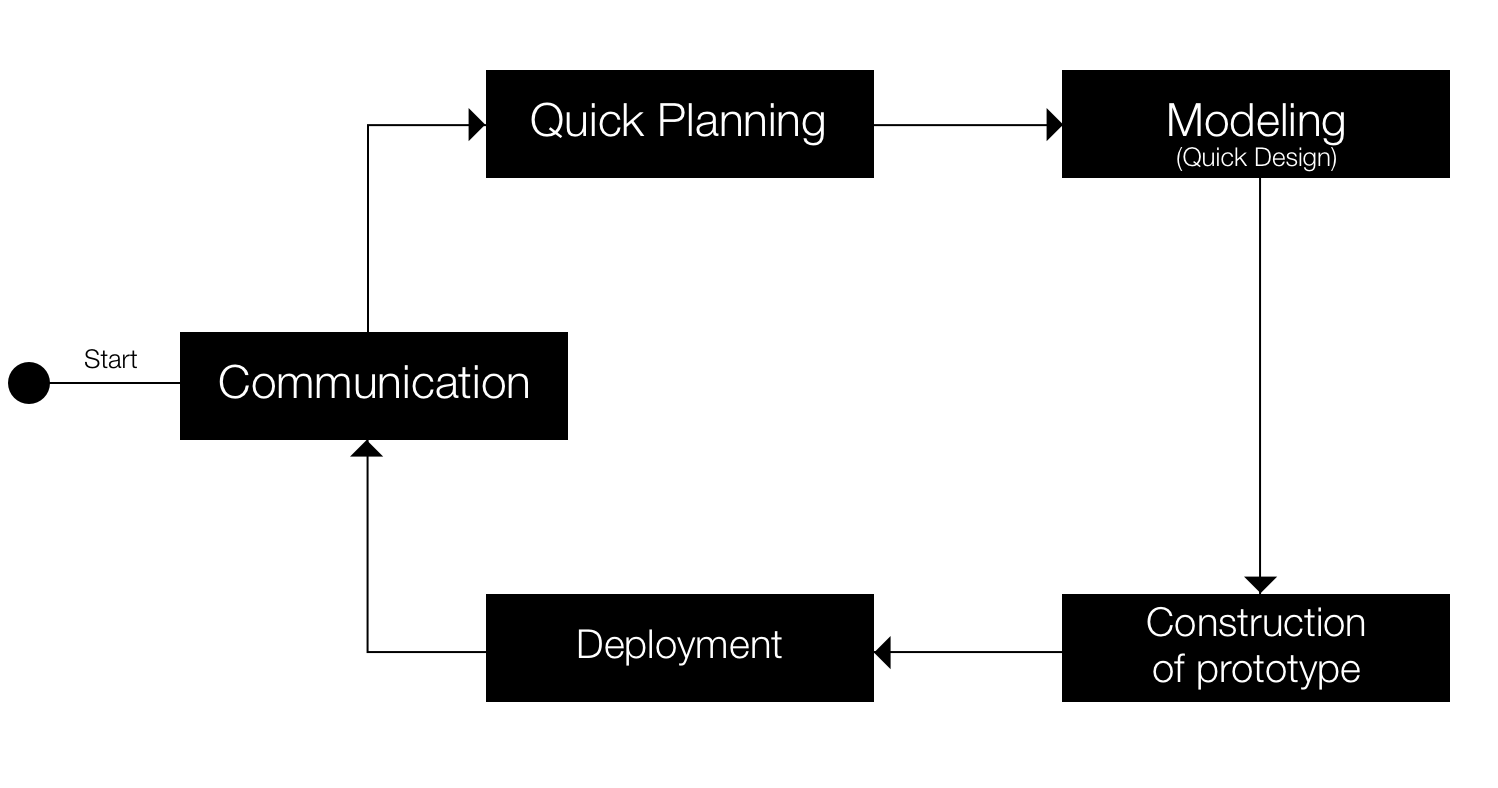
\includegraphics[scale=0.5]{Figures/PrototypingModel.png}
	\rule{35em}{0.5pt}
	\caption[Prototype Model Diagram]{Prototype Model Diagram}
\end{figure}

\pagebreak
\subsection{Reasons for choosing prototyping model}
By end of 2016 the population in Cyberjaya will be about 100,00, and most of people in Cyberjaya uses buses as their cheap and easy transportation method \cite{ReferencePopulationOfCyberjaya}. That makes MTS highly required and might be used by most of people who live in Cyberjaya. For that reason, bugs would be found easily and bugs would need a quick fix to reduce the damages and failures.\\

An advantage of Prototyping model is that the quicker user feedback is available which leads to better solutions and fast error fixing. In other words, users are actively involved in the development.\\

MTS is a system that needs to have interactions with the end users, therefore, Prototype model should be used. Moreover, MTS is an online system which has direct interfaces with many users at the same time. MTS might has a high amount of interaction with the end-users so prototype model is best compared to other models.\\